\section{CSP reporting analysis}

Part of my work was to evaluate the use of reporting within websites policies.

To aid me in my task NetCraft has provided me with a list of top 1 million sites.
I have requested their main pages and stored their CSP and CSPRO headers.
Later, I have scanned all policies for inclusion of reporting sources.
\texttt{report-to} and \texttt{report-uri} allow for CSP violations to be sent to the dedicated server.
Crucially their declaration is not supported in \texttt{<meta>} HTML tags within the source code of sites using CSP.

\subsection{Analysis Results}

From my analysis I observed that 14\% of websites that responded with a 200 OK response code were using some form of a CSP policy.
This shows a steady increase of CSP adoption by hosts compared to other studies and reports.
Unfortunately, through my analysis of the policies for reporting sources, I have observed that only 4\% of all policies allow for any form of reporting.

Similarly I have checked report only headers. 
Only 1\% of websites used a CSPRO header and out of those only 50\% included reporting endpoints.
Reporting only header does not change any behaviours of browsers. 
Knowing this, 50\% of hosts using a CSPRO header have it without getting any benefits of such header.

Out of 1 million sites tested, only 2881 sites reported using both active and reporting policies at the same time.
Many of those sites were various endpoints of the biggest hosts on the internet.
Through manual analysis, polices used here can be roughly split into 3 groups.

Similar, but with small changes.
For example, \texttt{instagram.com} report only policy disallows images to be loaded from \texttt{*.whatsapp.com}, which is allowed in the enforcement policy.
This method allows for sites to function as expected by users, but all occurrences of a specific media will be reported.
Using reporting only header in this way may allow for eventual removal of a dependency from the site.

There were significant number of host using enforcement mode for \texttt{frame-src} and \texttt{upgrade-insecure-requests} sources and report-only header for other uses of CSP like scripts, styles or images.
This approach allows for quick deployment of low cost directives which prevent data leaks through insecure connections and click jacking, two big attack vectors that CSP can help prevent.
While those basic security measures are in place, developers can focus on much more advanced and harder to properly create policy that included all the other directives.

Last group, most disappointing, had identical policies for both enforcement and report only modes.
Here I have observed this behaviour in 11\% of all servers running both headers.
This may be due to developers keeping the old report only header when moving to enforcement mode after creating a policy for their website.

\section{Automated policy maker}

With such low usage of \texttt{content-security-policy-report-only} header I decided to create an automated policy maker which would allow for increased utilization of this header leading to an increase in security.

\subsection{Ideology}

Although report only header does not limit any resources from being loaded, it can be used very well for monitoring purposes.
When using the standard \texttt{content-security-policy} header any attack bypassing the policy will never be reported as enforcing and reporting go hand in hand, leading to untraceable attacks.
In my approach I make a tool that is \"bypassable\" by default as it is not enforced, but instead it will always report on any potentially malicious script.
To help me develop my policy maker, which will be using the report only mode, it is critical to realize that I do not need to adhere to constraints of standard enforcing policies.

When using report only header I do not need the policy to contain all the loaded resources, that are used by the web application.
As the policy is not enforced and I do not risk breaking the application I may periodically remove certain sources to check whether they are still used.
In this way I always keep an up to date list of all resources used by the website.

Additionally, by using report only I do not need to make the policy work with possible updates.
Contrarily, I would like to get informed about any changes to scripts used as soon as possible.
I can accomplish this by using hashes as sources instead of standard url style allow lists.
As hashes are unique to the file, users will report to my server as soon as anything changes, allowing me to be immediately notified about potential threats.

\subsection{Development}

The project is mainly written in JavaScript and uses Node as runtime.
This combination was used as it provides high level, powerful and very customizable tools required for efficient server creation.
It also natively supports JSON data format, which is used for Content-Security-Policy reports.
Many tools used within this project are available in the Node Package Manager allowing for better interoperability.
Components that are not available under Node were connected, by creating separate servers which communicated using GET and POST requests.

The high level view of the project structure is desplayed in figure \ref{structure}.
The project uses mutliple interdependant modules, which expose limited amount of functions to support modularity.
The key development within this project is on the diagram denoted as the Policy Maker.
It is designed as a separate entity, which does not require the other components used within this project to function.
When deployed in a real environment, it may be directly connected to the server serving HTTP requets, while providing an up to date policy for the observed reports.
The Policy maker consists of 3 other smaller modules 
\begin{description}
	\item[Main server] Receives reports and generates policies
	\item[Oracle] Takes script urls from reports and aims and collects them from the internet
	\item[Evaluator] Rates collected scripts and evaluates them
\end{itemize}

% TODO
A set of other tools was used to support the server during the development and testing.
To simulate the control over the host, mitmproxy was used. 
Also Puppeteer was used to simulate the user over the extended period of time of testing, while also guaranteeing consistency between tests, 

\begin{figure}[H]
	\centering
	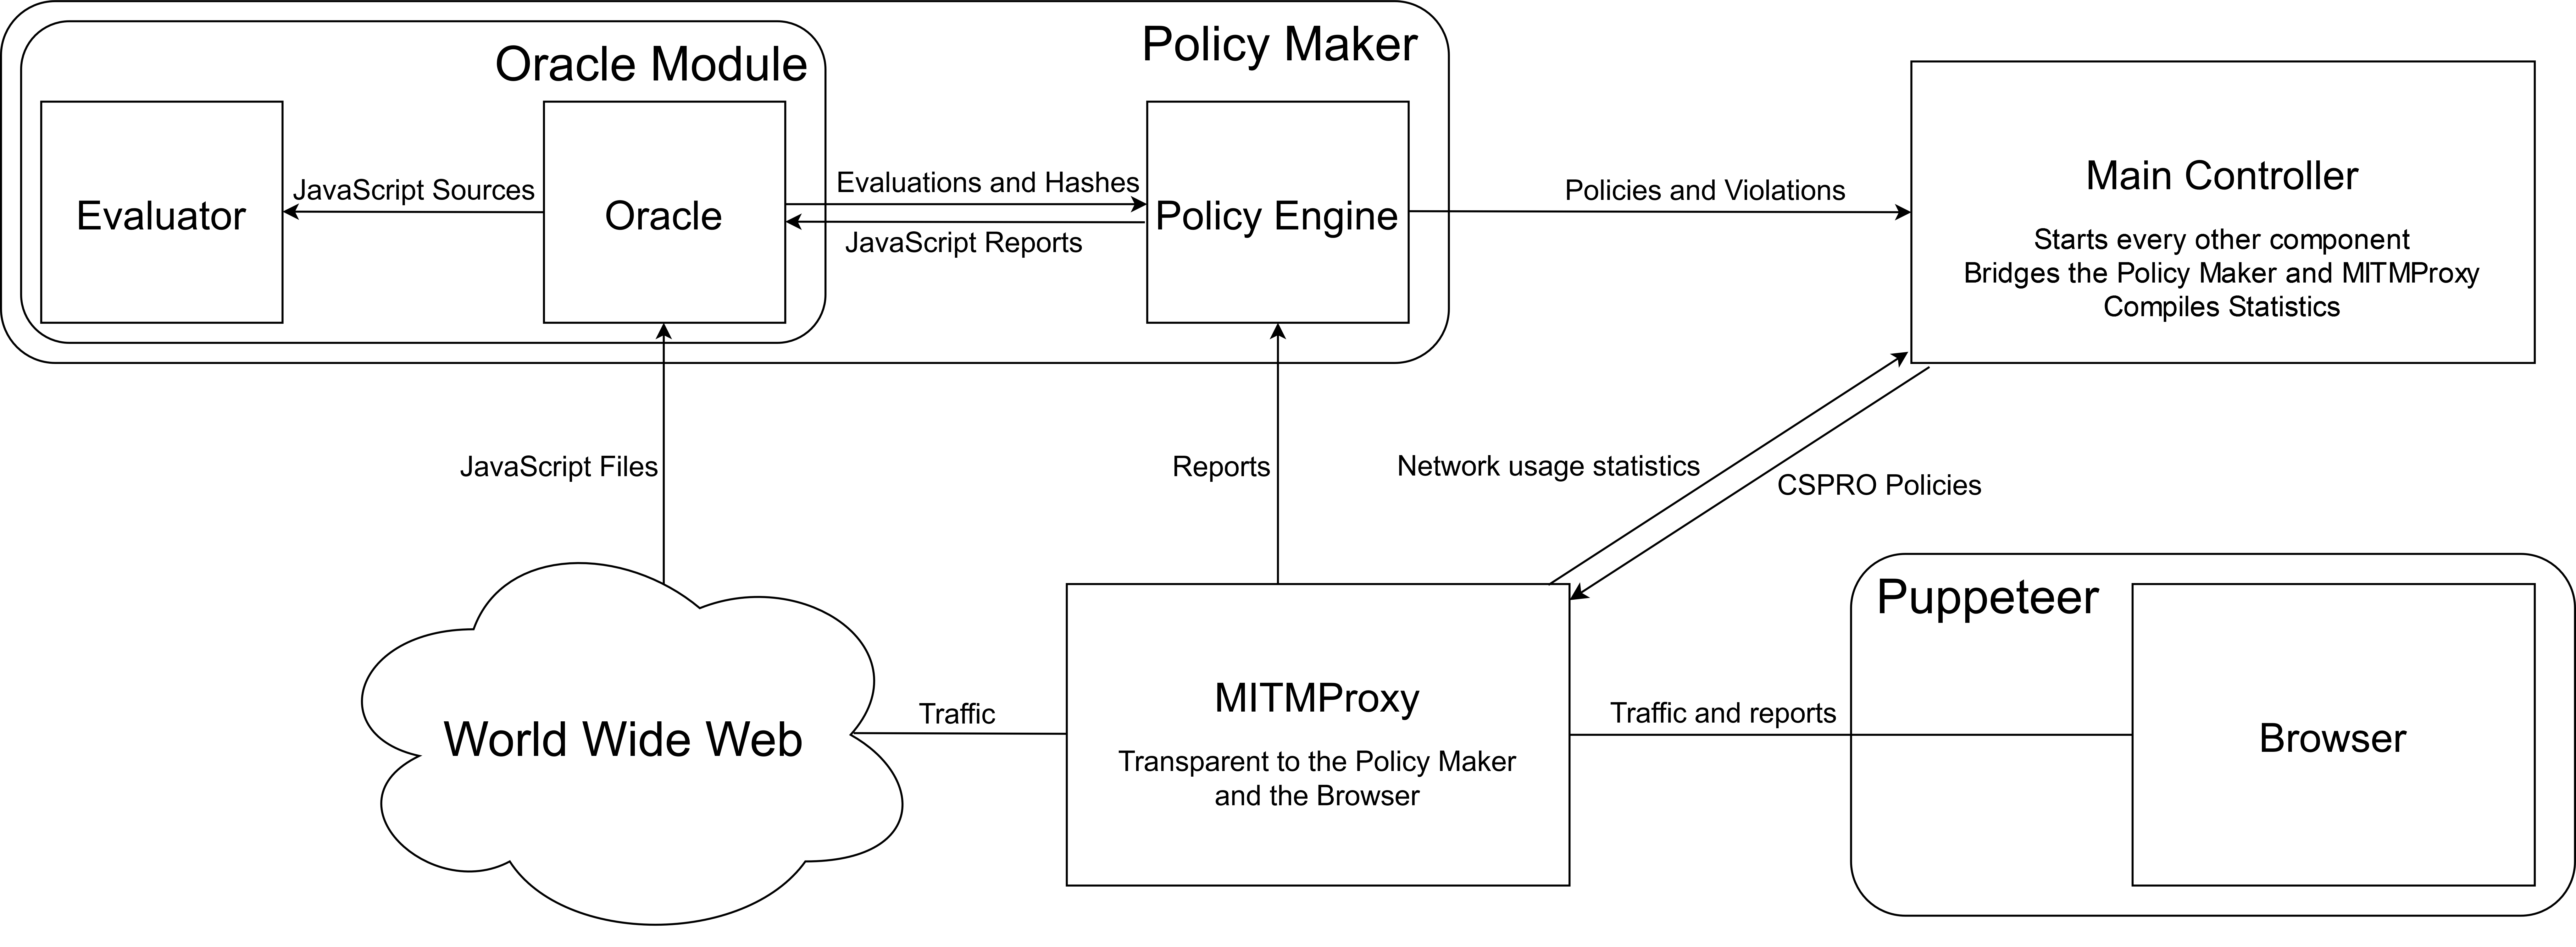
\includegraphics[width=\textwidth]{imgs/project_structure.png}
	\caption{Structure of the project}
	\label{structure}
\end{figure}

\subsubsection{Server}
The server is the main component which exposes and open port dedicated to collecting reports.
It is also the outermost layer of communication responsible for issuing warnings as they are encountered.
This module exposes an \texttt{EventEmitter} interface, which allows other components to run specific code when an event occurs.
There are 5 possible events, 2 for security, 2 for logging and 1 for CSP updates:
\begin{description}
	\item[\texttt{warning}]	Used to signify rarely used content which should be monitored. Practically it is used for iframes and small inline attribute scripts. 
	\item[\texttt{violation}] Uesd to signify malicious scripts, use of \texttt{eval} function or long attribute scripts that do not fit in the 40 character report limit.
	\item[\texttt{new}] Signifies a new script has been spotted.
	\item[\texttt{changed}] Signifies that a previously spotted script has been changed.
	\item[\texttt{cspro-change}] Emmitted whenever a policy is changed, notifying any module to update their CSPRO value.
\end{description}

When reports are received, they are parsed and the most important information is stored in the memory.
The full contents of the report are stored in a database alongsite the timestamp when they arrived.
Depending on the effective violated directive different actions are performed.
Sources like images, fonts or styles are premanently added to the policy, as this project focuses on securing web applications from malicious scripts.
Iframes trigger a warning event as they may be used for clickjacking attacks, after which they are added to the policy, as they are not the main focus of this paper.

The most logic within the server is dedicated to scripts.
Attribute scripts always trigger a warning or a violation event.
Then depending whether they fit into the 40 character limit within the \texttt{script-sample} field in the report, their hash may be added to the policy for a short duration to limit the amount of duplicate reports.
Reports signifying use of \texttt{eval} function emit a violation event, after which they are ignored.
Lastly all reports about scripts within HTML \texttt{<script>} tags are sent to the oracle to calculate their hash and evaluate their maliciousness.
All hashes are stored and based on them the server recognises whether a script has changed and in that case it emits a changed event.

\subsubsection{Oracle}
The oracle is the inner module of the Policy Maker which is crucial for the functionality of the server.
Its main goal is to aid the server in collecting scripts described in reports and to provide their evaluation.
The oracle is a separate module to allow for a redesign without affecting the core logic of the server.
In this project scirpts are fetched from the hosts using GET requests, but this mechanism could be adjusted to instead fetch specific scripts from the inner code repository.

\subsubsection{Evaluator}
The evaluator in the Oracle Module is used to evaluate scripts from the sourcecode that was collected by the oracle.
Compared to the oracle it is not necessary for the function of the Policy Maker, but without one only new and changed events will be emitted.
The evaluator included in the source code uses a machine learning model created by Maria Zorkaltseva intended to find obfuscated malicious JavaScript files \cite{evaluator}.
As the model is written in Python, downloaded scripts are passed to a python http server using POST requests.
The server calculates the maliciousness score and returns the result in the response.


% TODO
The server additionally uses PostgreSQL to store reports and responses from the oracle.
Data is logged in the database for safe-keeping, post-deployment analysis and debugging.
Additionally the collected reports can be reused to repeat the experiments on the same data, it also reduces the strain this project exerts on websites I am using to test my algorithm.


\subsubsection{Main Controller}
Main Controller is the entry module for the project.
Every other module described requires a context for its execution.
The main controller sets up each module with a context required to run a specific test scenario.
It collects all events emited from the server and logs them to the console for a clear view of the servers operation.
Whenever a new policy is generated, the main controller passes it from the server to the mitmproxy so it can be injected into server responses.
Lastly the main controller logs statistical data collected by mitmproxy.


\subsubsection{Mitmproxy}
Mitmproxy is an interactive https proxy which can be used to intercept, read and modify traffic coming through it.
It supports scripting, which is used to automatically insert \texttt{content-security-policy-report-only} header before it is sent to the browser.
In this way, the browser sees the modified response as if it was sent directly from the host.
This behaviour directly emulates the scenario where the policy maker were to be deployed alongside the hosting server.
As all traffic is directed through mitmproxy, it has also been used to collect statistics required to evaluate the project.
In the code this integration works by creating a separate server to which the mitmproxy module connects periodically.
Whenever this happens all data collected is sent away and a current CSPRO generated by the reporting server is returned.
Due to this design there is slight latency between generation of a new policy and deployment to the user.
Although this delay exists, it is insignificant and in real world many hosts use proxies to reduce the load on servers or clients use caching to reduce their network usage.
In both of those cases the delay between deployment of a new CSPRO and its perceivable effects may be much larger than what is observed in this project and as such this issue is ignored throughtout the testing.


\subsubsection{Puppeteer}
The second tool used that does not benefit the security of the server, but was extensively used during testing was Puppeteer.
Puppeteer is a Node.js module designed to simulate user interaction in a chromium client.
It uses a programmable interface, which results in high precision and reproducability between executions.
For those reasons Puppeteer was used for all impact estimation tests.
In the code a separate module was dedicated to Puppeteer which starts it up connected to the proxy with parameters simulating a regular user.
After that it is used to crawl the currently tested host.


\section{Initial Content-Security-Policy}

During development of the server I have faces multiple choices relating to the initial CSPRO header, which is set before any report is even received.
There are a few sources which dramatically change the behaviour of browsers enforcing the security policy, which impact security or the threat surface that I may protect against.

\subsection{unsafe-inline}

\texttt{unsafe-inline} allows all inline scripts to execute. 
This source is disincentivized by Mozilla Docs \cite{unsafeinlinebad2} and CSP Quick Reference Guide \cite{unsafeinlinebad1}.
It is also shown to be insecure in multiple papers \cite{weichselbaum2016csp} \cite{osti_10173479}.

This is largely due to the fact that it allows for dynamic execution of scripts, by inserting them directly into the website code.
It also prevents any reports to be generated in case of a DOM injection attack.

I was considering using \texttt{unsafe-inline}, as my oracle uses a best effort approach to extracting inline scripts.
This leads to many scripts being unable to be extracted without executing the loader script.
I have decided that executing unknown scripts is very unsafe and consequently my server will never be able to know the source code or the hash.
It means that the browser will always send a report to my server whenever a script is loaded in this way, impacting the performance.

In the end I believe that although there are practical implications to including \texttt{unsafe-inline} source into the CSP, it has too severe negative implications.
The CSP becomes easily bypassable and 

\subsection{self}

Adding \texttt{'self'} to the source list of scripts would allow for all scripts coming from the host to be executed without sending the report.
It still sends a report for every inline script and it  may be a good option for a host that employs many security measures towards its own code.
When used it reduces the amount of reports and reduces the average size of the report as none of sites own scripts will need a hash to execute.
This method successfully changes the threat surface from all scripts used on a web application to monitoring changes only in external scripts.

In my experiments I do not use \texttt{'self'} source as I my aim was to develop a policy maker that is as secure as possible.
The change is the threat surface is big enough where a fully automatic system should be able to protect agains insider threat.

\subsection{strict-dynamic}

\texttt{strict-dynamic} is a successor to \texttt{unsafe-inline}, where it will allow dynamically loaded scripts as long as they are loaded from a script that is allowed by a nonce of a hash.
It also changes the behaviour of the policy where it instructs the browser to ignore \texttt{unsafe-inline}, \texttt{'self'}, \texttt{unsafe-eval} or many other wildcard statements.

When using \texttt{strict-dynamic} I am still unable to gather hashes for dynamically loaded scripts, but in this case, those scripts will not send reports about an inline script being used, partially mitigating the issue.
Similarly, non-inline dynamically added scripts will also not generate a report, which I would be able to retrieve, evaluate and generate a hash for.
For this reason I do not use \texttt{strict-dynamic} source as it still undermines the security of my solution.

\subsection{unsafe-hashes}

Adding \texttt{unsafe-hashes} to the source list allow for hashes to be used for inline scritp attributes such as \texttt{onClick} or \texttt{onLoad}.
It uses the prefix {\it unsafe}, but hashes in \texttt{script-src-attr} directive by default are ignored as they will never have a valid target to allow.
As such I only use \texttt{unsafe-hashes} for this specific directive. 
Also I only use it for scripts that fully fit in the 40 character limit dedicated to the script sample field in the report and I always generate a violation event for such a report.

\section{Evaluation}

The automated policy maker is evaluated in this work by the methods of empirical tests, which show that the program is working correctly.
This work also aims to estimate the impact of deploying the solution in the real world.
This set of tests compares the network impact of the solution to the loads that the hosts are already experiencing in their normal operation.

\subsection{Empirical tests}

This project consists of multiple modules which all work together to achieve a bigger goal.

Oracle is a module that is used to generate hashes of loaded resources and communicate to the python evaluation server.
When tested on a local server, it can successfully fetch files from it and generate hashes equal to the ones that are generated with system tools on file data.
After receiving line and file information it is sometimes able to extract data from inline scripts embeded in the html of the page.
Ocasionally, due to formatting, encoding or other issues related to dynamic inclusion of data into the page, it may return no or a wrong hash.
Due to security concerns my oracle does not dynamically execute scripts and change html code, which does happen within the browser.
Most notably a script may change the inner html of a page to one with another script.
In this case the oracle is unable to generate the script that was included as it is not included in the retreived html.
Throughout testing of this project, different scripts responsible for advertisements and user tagging were found to use this technique.
The influence that those scripts have on the effectiveness of this project will be clearly seen when the impact of the cspro server is estimated.

The second role of the oracle is to pass the script extracted to the evaluation server.
When a script is passed to the evaluator a simple binary response is returned representing whether the script was found to be malicious.
As this work focuses mainly on developing the policy maker for CSPRO header and the evaluator is a machine learning model described in a different paper, its functioning is not thoroughly tested.
While its results may be occasionally inaccurate, it still clearly demonstrates the inner workings of the Policy Maker server.

The server which is the main outcome of this project uses the oracle extensively.
Each script that is reported are sent through the oracle, then depending on the evalutaion they are added to the policy for a specific amount of time.
Eventually after enough time has passed the server succesfully removes the entry from its policy.
When a new report for the same resource arrives it compares the new evaluation from the oracle to the previous one and does emit events related to the result.
Each time the CSPRO value is changed it is communicated out of the server and subseqently embedded into html responses by mitmproxy.

During testing this result is eaily observable in the browser connected to the proxy.
When loading the host page on a newly created server, multiple reports are generated back to the server.
On the server multiple new events can be seen and in a case where there is a script deemeed malicious a violation is observed too.
Subseqeunt refreshes of the page in the browser no longer produce reports until the scripts present are removed from the policy.
Even if there are more reports arriving the server will not generate new events unless a scripts has changed.

The server also keeps note of other resources loaded on the page with a lower level of detail.
It stores only hosts of those resources, which are added to the policy of the server and they are not removed over time.
When a new source is added only the update of the CSPRO is triggered, but no additional event is emitted.

The only exception to this rule the \texttt{frame-src} directive. 
When a report about a violation to the frame-src is received a new warning is emmited.
As previously described iframes can be used in clickjacking attacks and due to lower amount of iframes used on pages it is important to verify that no malicious iframes are running.

After testing the server on a model webiste a Content-Security-Policy-Report-Only header has been generated that encapsulates all the described behaviours.

% TODO add CSPRO HEADER

And the server had emmited the following events.

% TODO add events

\subsection{Impact estimation}

To try to provide most accurate results I have tried to deploy my solution on a mixture of randomly selected hosts from top 10,000 hosts and a few which would most likely be interested in deploying such protection method.

In this paper I present results gathered from 4 websites, which I believe provide a broad range of results as well as demonstrate some issues where my solution is unlikely to be beneficial.
None of the sites which were used to test the policy maker have deployed their own CSP or CSPRO headers.
This was done to avoid the policy overwritten in the proxy to be further modified by the meta tags included in the page source.
Choosing such sites would also skew the results as those websites would already have been adjusted to work with CSP.

During the tests the server is deployed seperately on all the described hosts.
In each of the tests a set of 171 subpages are opened over a timespan of 45 minutes. 
The first page opened is always the mainpage for the host, after which a random page is chosen out of all anchor links seen throughout the test.
For the tests the server will remove a JavaScript link after 10 minutes.

As this tests are done on real hosts it is impossible to assume maliciousness of any of the scripts returned as malicious.
From all of the reported scripts that were analised by hand, the most common issues for those reports were dubious programming practices or unnecessary obfuscation of seemingly banign scripts.

% talk how data is collected in mitmproxy


\subsection{www.libertatea.ro}

\texttt{www.libertatea.ro} is a Romanian news website which I have found to be possibly the worst web-app to deploy my server on.
They are dynamically loading many scripts, making it near impossible to retrieve the executed scripts.
With this behaviour I am unable to rate the scripts as well as assign the hash that is being used to add to my \texttt{CSPRO} header.

Due to those dynamically loaded scripts, the site transfers 9 times more data in reports back to my server than what was originally sent from \texttt{www.libertatea.ro}.

I could prevent this behaviour by using \texttt{'strict-dynamic'} source in scripts directive, which would result in all loaded scripts to be allowed to run, as long as the loader is allowed by the hash.
This solution although would reduce the amount of reports sent, would instead result in drastic reduction in security as my server no longer has a proper worldview on the application.
In such case, if one of the loader sites became compromised and started sending malicious scripts to load, I would be unable to detect such change.

\subsection{quran.com}

\texttt{quran.com} is a digital provider of Quran. 
This website is another example of a host that would prove impossible to implement the server described in this paper.
The application sends a unique JavaScript file for each verse of Quran, as those files contain the data that is shown to the user.
As each of those files has a unique path the policy generated by the server will grow to and unmaintainable size.

In the case of this site, the best solution would be to seperate the data part of the scripts into their own fetchable json files.
When a file is retrieved from the web by a script it falls under \texttt{connect-src} directive. 
Only after including the data into the website more reports will be generated depending on the data included.
Hopefully little to none additional scripts would be included to avoid this circular dependency.
After this change only the script with its full path will be in the script directive, while the connect directive will include only the host from which all the data is coming from.
This will both allow for good security and minimization of the CSPRO header.

% default-src from prefetching ?

\subsection{www.professormesser.com}

Professor Messer is a group dedicated to providing teaching courses and resources related to technical certificates.
This website shows good results in shoert term deployment, but due to dynamically loaded scripts performs poorly during longer tests.


\subsection{www.caixabank.es}

As all randomly chosen hosts proved to show no good results \texttt{www.caixabank.com} was as an example of a site that may already be interested in security and avoids the pitfalls of the previous hosts.
It is the only hand picked site that this project was ever tested on. 
It has much better results, but still shows that deploying such a server would require a significant amount of resources.
Towards the end of the experiment an extensive policy was created, yet the site still generated reports due to use of \texttt{eval} function in their code.

Eval is a notoriously unsafe function used very often in malicious scripts. 
It allows for execution of any string of characters to be executed as a JavaScript code. 
In Content-Security-Policy this function is seperately recognised with its own source directive for scripts: \texttt{unsafe-eval}.
The reports also use a unique value of \texttt{eval} in their \texttt{blocked-uri} field.
The only way to stop those reports without changing the pages source is to add \texttt{unsafe-eval} to the script sources.
Unfortunately in that way all malicious uses of \texttt{eval} function are also omitted.
Due to that \texttt{unsafe-eval} is never added to the policy and through countless violations emitted by the server, the developers may be included to stop their bad practices and refactor the code.

\subsection{Test results}

All of the websites on which the automated policy maker was tested show limited value to be gained from such an automated tool.
This comes from a fact that a security measure that aims to keep track of all the systems running on a web application is too resource intensive.
While consuming too much resources it also may not increase the security of those sites substantially due to already very wide attack surface.


Despite poor performace on these selected hosts, the work done in this paper can still be beneficial to smaller endpoints which already put in significant amount of work to insure the security of thier website.
Ceixabank was used to see what an exaple of potentially such website could be, as customers of a bank would expect utmost security, especially after logging into their online services.
Even though they may use a different subdomain after a user is logged in, it is still disappointing to see \texttt{eval} function being commonly used.


\begin{figure}[h]
	\centering
	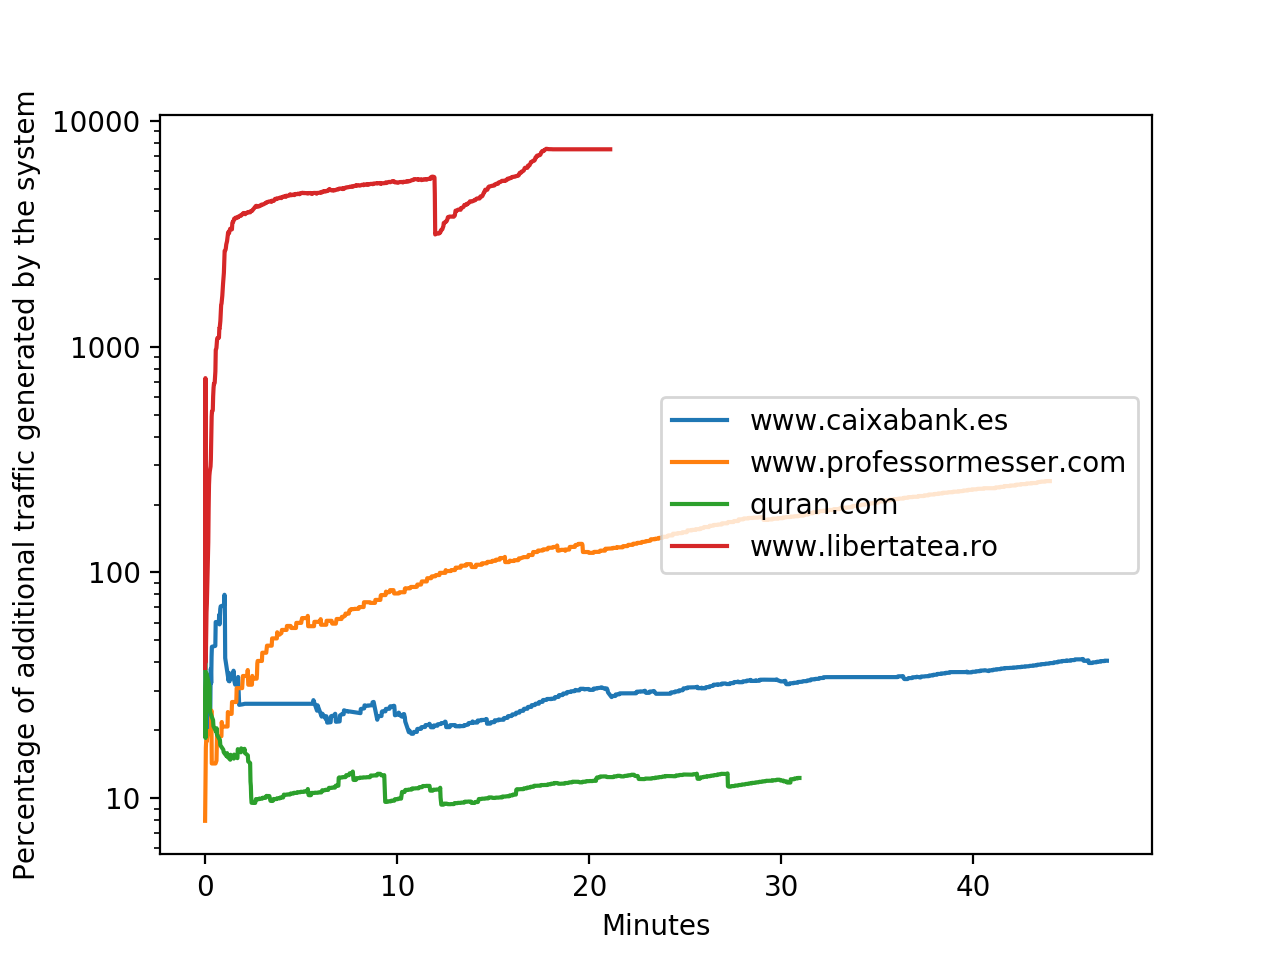
\includegraphics[width=\textwidth]{imgs/netword_usage_plot.png}
	\caption{Percentage of bandwidth dedicated to additional traffic generated by my policymaker}
\end{figure}


\section{Discussion}

% What is a good time to forget the link

\section{Things to improve}

My approach shows to be a promising and new way to improve the security of particular websites.
Main applicability issues stem from the quickly expanding and untamed environment of front end development.

Things that could dramatically improve the performance of my policy maker would require changing the CSP standard.
Allowing for more control over the report template could reduce the data transferred back to the CSP reporting endpoint by at least 90\%.
This comes from each report containing the current policy used when loading the page, which is responsible for most of the traffic.

I would like to have more control over the report where I could specify the browser to pass the script hash back to me.
I believe it could be implemented in a similar way to \texttt{report-sample} source, where \texttt{report-hash} would send the hash of the script as received by the browser.
This would speed up the recognition of changes resources. 
Currently my server caches the resources and it would recheck and reevaluate the source only after a certain period of time has passed.
If a hash were to be passed alongside the \texttt{blocked-uri} field I could immediately recognise any changes.
This would further improve the security as timeouts may be troublesome to adjust between possibly not seeing every change and unnecessarily retrieving the same file over and over again.

Within my own approach, further development of an oracle to judge scripts is crucial to reap full benefits of this system.
I do not introduce new breakthroughs in script detection, but merely use what I have found to be fit for my purpose.
The oracle that I am using very often tags ad scripts as malicious, as they do load variable content onto the website and due to that use many functions commonly found in malicious scripts.

Within my work I try to show that improving the defence of websites is feasible by introducing an automatically generated policy, but I never implement it on any website with real users.
The next big step in proving the functionality of this approach would be to test it on a real host.
There many issues would need to be resolved similar to the issues that relate to deploying a standard CSP.
Users may embed or block scripts by using external plugins. 
My server could detect those by knowing from the development environment which scripts are expected to be loaded by the end users. 

Through my tests I have also used only a single browser.
Although all browsers available to my Linux testing environment have functionally identical reporting, I have not tested on outdated and mobile browsers.
Testing my solution in the wild would also resurface many issues related to the complexity of end environments.k

% talk about malicious iframe detection
